\documentclass[aspectratio=169,10pt]{beamer}
\usepackage[T1]{fontenc}
\usepackage[utf8]{inputenc}
\usepackage[french]{babel}
\usepackage{lmodern}
\usepackage{booktabs}
\usepackage{graphicx}
\usepackage{amsmath}
\usepackage{xcolor}

\usetheme{Madrid}
\setbeamertemplate{navigation symbols}{}
\setbeamertemplate{caption}[numbered]
\setbeamertemplate{blocks}[rounded][shadow=false]

\definecolor{bleu}{RGB}{13,71,161}
\definecolor{bleufonce}{RGB}{10,45,105}
\definecolor{bleuclair}{RGB}{227,239,252}
\definecolor{orange}{RGB}{224,148,0}
\definecolor{gris}{RGB}{90,90,90}

\setbeamercolor{structure}{fg=bleu}
\setbeamercolor{palette primary}{bg=bleu,fg=white}
\setbeamercolor{palette secondary}{bg=bleufonce,fg=white}
\setbeamercolor{palette tertiary}{bg=bleufonce,fg=white}
\setbeamercolor{title}{fg=white}
\setbeamercolor{subtitle}{fg=white}
\setbeamercolor{frametitle}{bg=bleu,fg=white}
\setbeamercolor{block title}{bg=bleuclair,fg=bleufonce}
\setbeamercolor{block body}{bg=bleuclair!45,fg=black}
\setbeamercolor{itemize item}{fg=bleu}
\setbeamercolor{itemize subitem}{fg=bleu}
\setbeamertemplate{itemize item}{\small$\blacktriangleright$}
\setbeamertemplate{itemize subitem}{--}

\setbeamertemplate{footline}{%
  \leavevmode\hbox{%
    \begin{beamercolorbox}[wd=.33\paperwidth,ht=2.4ex,dp=1.2ex,center]{author in head/foot}%
      \usebeamerfont{author in head/foot}\insertshortauthor
    \end{beamercolorbox}%
    \begin{beamercolorbox}[wd=.34\paperwidth,ht=2.4ex,dp=1.2ex,center]{title in head/foot}%
      \usebeamerfont{title in head/foot}\insertshorttitle
    \end{beamercolorbox}%
    \begin{beamercolorbox}[wd=.33\paperwidth,ht=2.4ex,dp=1.2ex,center]{date in head/foot}%
      \usebeamerfont{date in head/foot}\insertframenumber\,/\,\inserttotalframenumber
    \end{beamercolorbox}}%
  \vskip0pt%
}

\newcommand{\src}[1]{\vspace{0.1em}{\scriptsize\color{gris}#1}}
\newcommand{\MUSD}{\,\text{M USD}}

\title[Barrières tarifaires et exportations]{Barrières tarifaires et exportations marocaines de tomates}
\subtitle{Droits NPF, concentration des marchés et flux, 2010--2023}
\author[H.~Yacoubi \& M.~Ninia]{Hiba Yacoubi\\[0.25em]Meriem Ninia}
\institute{ENCG Settat --- Master Commerce International\\Projet 35 --- Data Science}
\date{Année universitaire 2026--2027}

\begin{document}

\begin{frame}[plain]
  \titlepage
\end{frame}

\begin{frame}{Contexte économique}
  \begin{columns}[T,onlytextwidth]
    \begin{column}{0.55\textwidth}
      \begin{itemize}
        \item Les exportations de tomates fraîches (HS 0702) sont
              majoritairement destinées au marché européen.
        \item L'accord d'association UE--Maroc (2000) prévoit des quotas
              tarifaires préférentiels hors saison européenne.
        \item Les droits NPF varient de 0\,\% (Émirats) à 15\,\%
              (Russie), avec des paliers saisonniers dans l'UE
              (0 / 8,8 / 14,4\,\%).
        \item Le Brexit (2021) place le Royaume-Uni à 11,1\,\% de droit NPF
              tout en lui laissant 10,3\,\% des flux.
      \end{itemize}
    \end{column}
    \begin{column}{0.42\textwidth}
      \begin{block}{Enjeu}
        Classer les marchés par niveau de protection, puis mesurer ce que
        les données publiques permettent réellement de conclure.
      \end{block}
      \begin{block}{Chiffres clés}
        \begin{tabular}{lr}
          \toprule
          Observations (Comtrade) & 506 \\
          Partenaires nommés & 80 \\
          Période & 2010--2023 \\
          Valeur cumulée & 8,95 Md\$ \\
          Part de l'UE & 83,4\,\% \\
          \bottomrule
        \end{tabular}
      \end{block}
    \end{column}
  \end{columns}
\end{frame}

\begin{frame}{Question de recherche et hypothèses}
  \begin{block}{Question de recherche (catalogue, Projet 35)}
    Quels marchés pratiquent les droits les plus élevés sur les tomates
    marocaines, et comment ces droits s'articulent-ils avec les flux ?
  \end{block}
  \vspace{0.6em}
  \begin{columns}[T,onlytextwidth]
    \begin{column}{0.32\textwidth}
      \begin{block}{H1}
        Les droits élevés réduisent les exportations vers les marchés
        protégés.
      \end{block}
    \end{column}
    \begin{column}{0.32\textwidth}
      \begin{block}{H2}
        La proximité géographique et la taille du marché expliquent
        l'essentiel de la répartition.
      \end{block}
    \end{column}
    \begin{column}{0.32\textwidth}
      \begin{block}{H3}
        La relation tarifs--exportations n'est pas linéaire
        (effets de seuil).
      \end{block}
    \end{column}
  \end{columns}
  \vspace{0.6em}
  \textbf{Objectifs :} classer les marchés, comparer quatre modèles avec
  validation temporelle, et documenter honnêtement ce que les données ne
  permettent pas de dire.
\end{frame}

\begin{frame}{Données et méthodologie}
  \small
  \setlength{\itemsep}{0.25em}
  \begin{columns}[T,onlytextwidth]
    \begin{column}{0.48\textwidth}
      \textbf{Quatre sources publiques, toutes tracées}
      \begin{itemize}
        \item \textbf{UN Comtrade} : exportations Maroc, HS 0702,
              2010--2023 (506 obs., 80 partenaires nommés).
        \item \textbf{Banque mondiale} : PIB courant
              \texttt{NY.GDP.MKTP.CD} (85,8\,\% couvert).
        \item \textbf{WITS / UNCTAD TRAINS} : droits NPF HS 070200
              (246 obs., 98,2\,\% de la valeur).
        \item \textbf{CEPII} : distances bilatérales (97,0\,\% couvert).
      \end{itemize}
      \textbf{Aucune donnée simulée, aucune imputation}
      \begin{itemize}
        \item Réponses HTTP mises en cache : pipeline rejouable.
        \item Métadonnées d'extraction (URL, date, licence) conservées.
      \end{itemize}
    \end{column}
    \begin{column}{0.48\textwidth}
      \textbf{Découpage temporel strict}
      \begin{center}
      \small
      \begin{tabular}{llr}
        \toprule
        Ensemble & Années & Obs. \\
        \midrule
        Entraînement & 2010--2019 & 272 \\
        Validation & 2020--2021 & 71 \\
        Test & 2022--2023 & 84 \\
        \bottomrule
      \end{tabular}
      \end{center}
      \vspace{0.2em}
      \textbf{Quatre modèles comparés}
      \begin{itemize}
        \item Référence 1 : moyenne historique.
        \item Référence 2 : régression simple (PIB).
        \item Modèle 1 : Ridge ($\alpha$ choisi sur validation).
        \item Modèle 2 : forêt aléatoire.
      \end{itemize}
    \end{column}
  \end{columns}
  \par\vspace{0.6em}
  \src{Validation temporelle obligatoire : le modèle ne voit jamais le futur.}
\end{frame}

\begin{frame}{Analyse exploratoire : évolution des exportations}
  \centering
  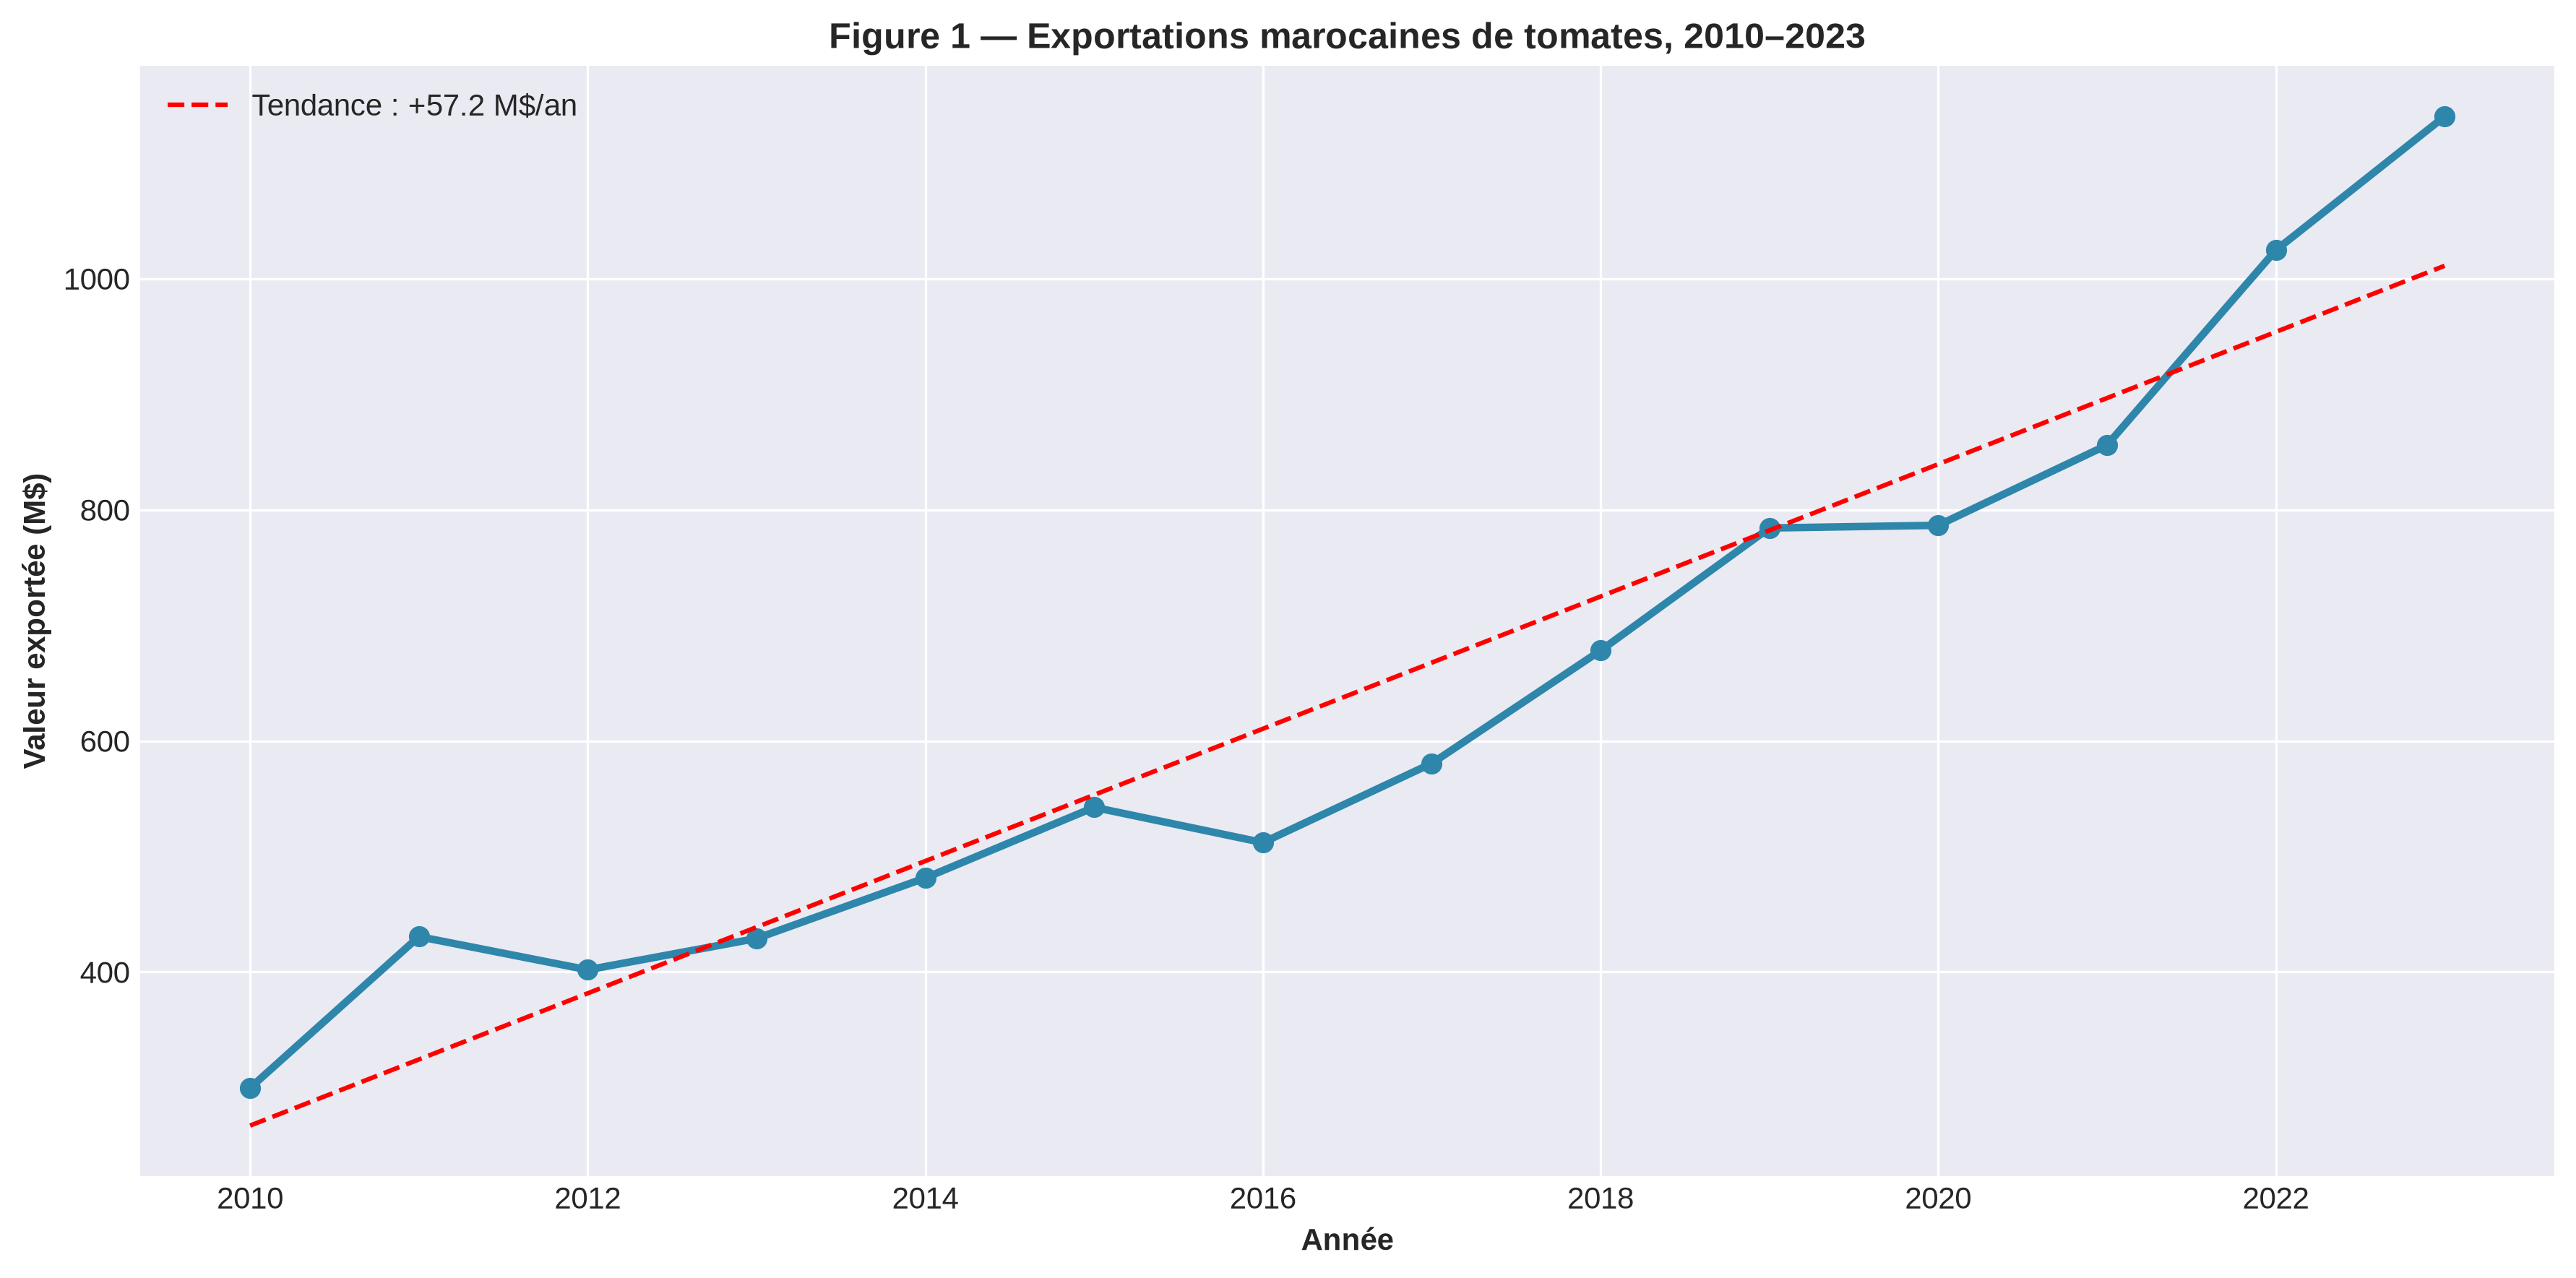
\includegraphics[height=0.56\textheight,width=\textwidth,keepaspectratio]{../figures/fig1_evolution_temporelle.png}
  \vspace{0.3em}

  \begin{columns}[T,onlytextwidth]
    \begin{column}{0.48\textwidth}
      \small
      \begin{itemize}
        \item $299{,}7$\MUSD{} (2010) $\rightarrow$ $1\,140{,}3$\MUSD{} (2023).
        \item Croissance de $+280\,\%$, soit $10{,}8\,\%$/an.
      \end{itemize}
    \end{column}
    \begin{column}{0.48\textwidth}
      \small
      \begin{itemize}
        \item Pas de rupture en 2020 : $786{,}5$ contre $784{,}2$\MUSD{} en 2019.
        \item La demande européenne en contre-saison a résisté.
      \end{itemize}
    \end{column}
  \end{columns}
  \src{Source : UN Comtrade, reporter 504, HS 0702 (figure~1 du rapport).}
\end{frame}

\begin{frame}{Analyse exploratoire : concentration géographique}
  \centering
  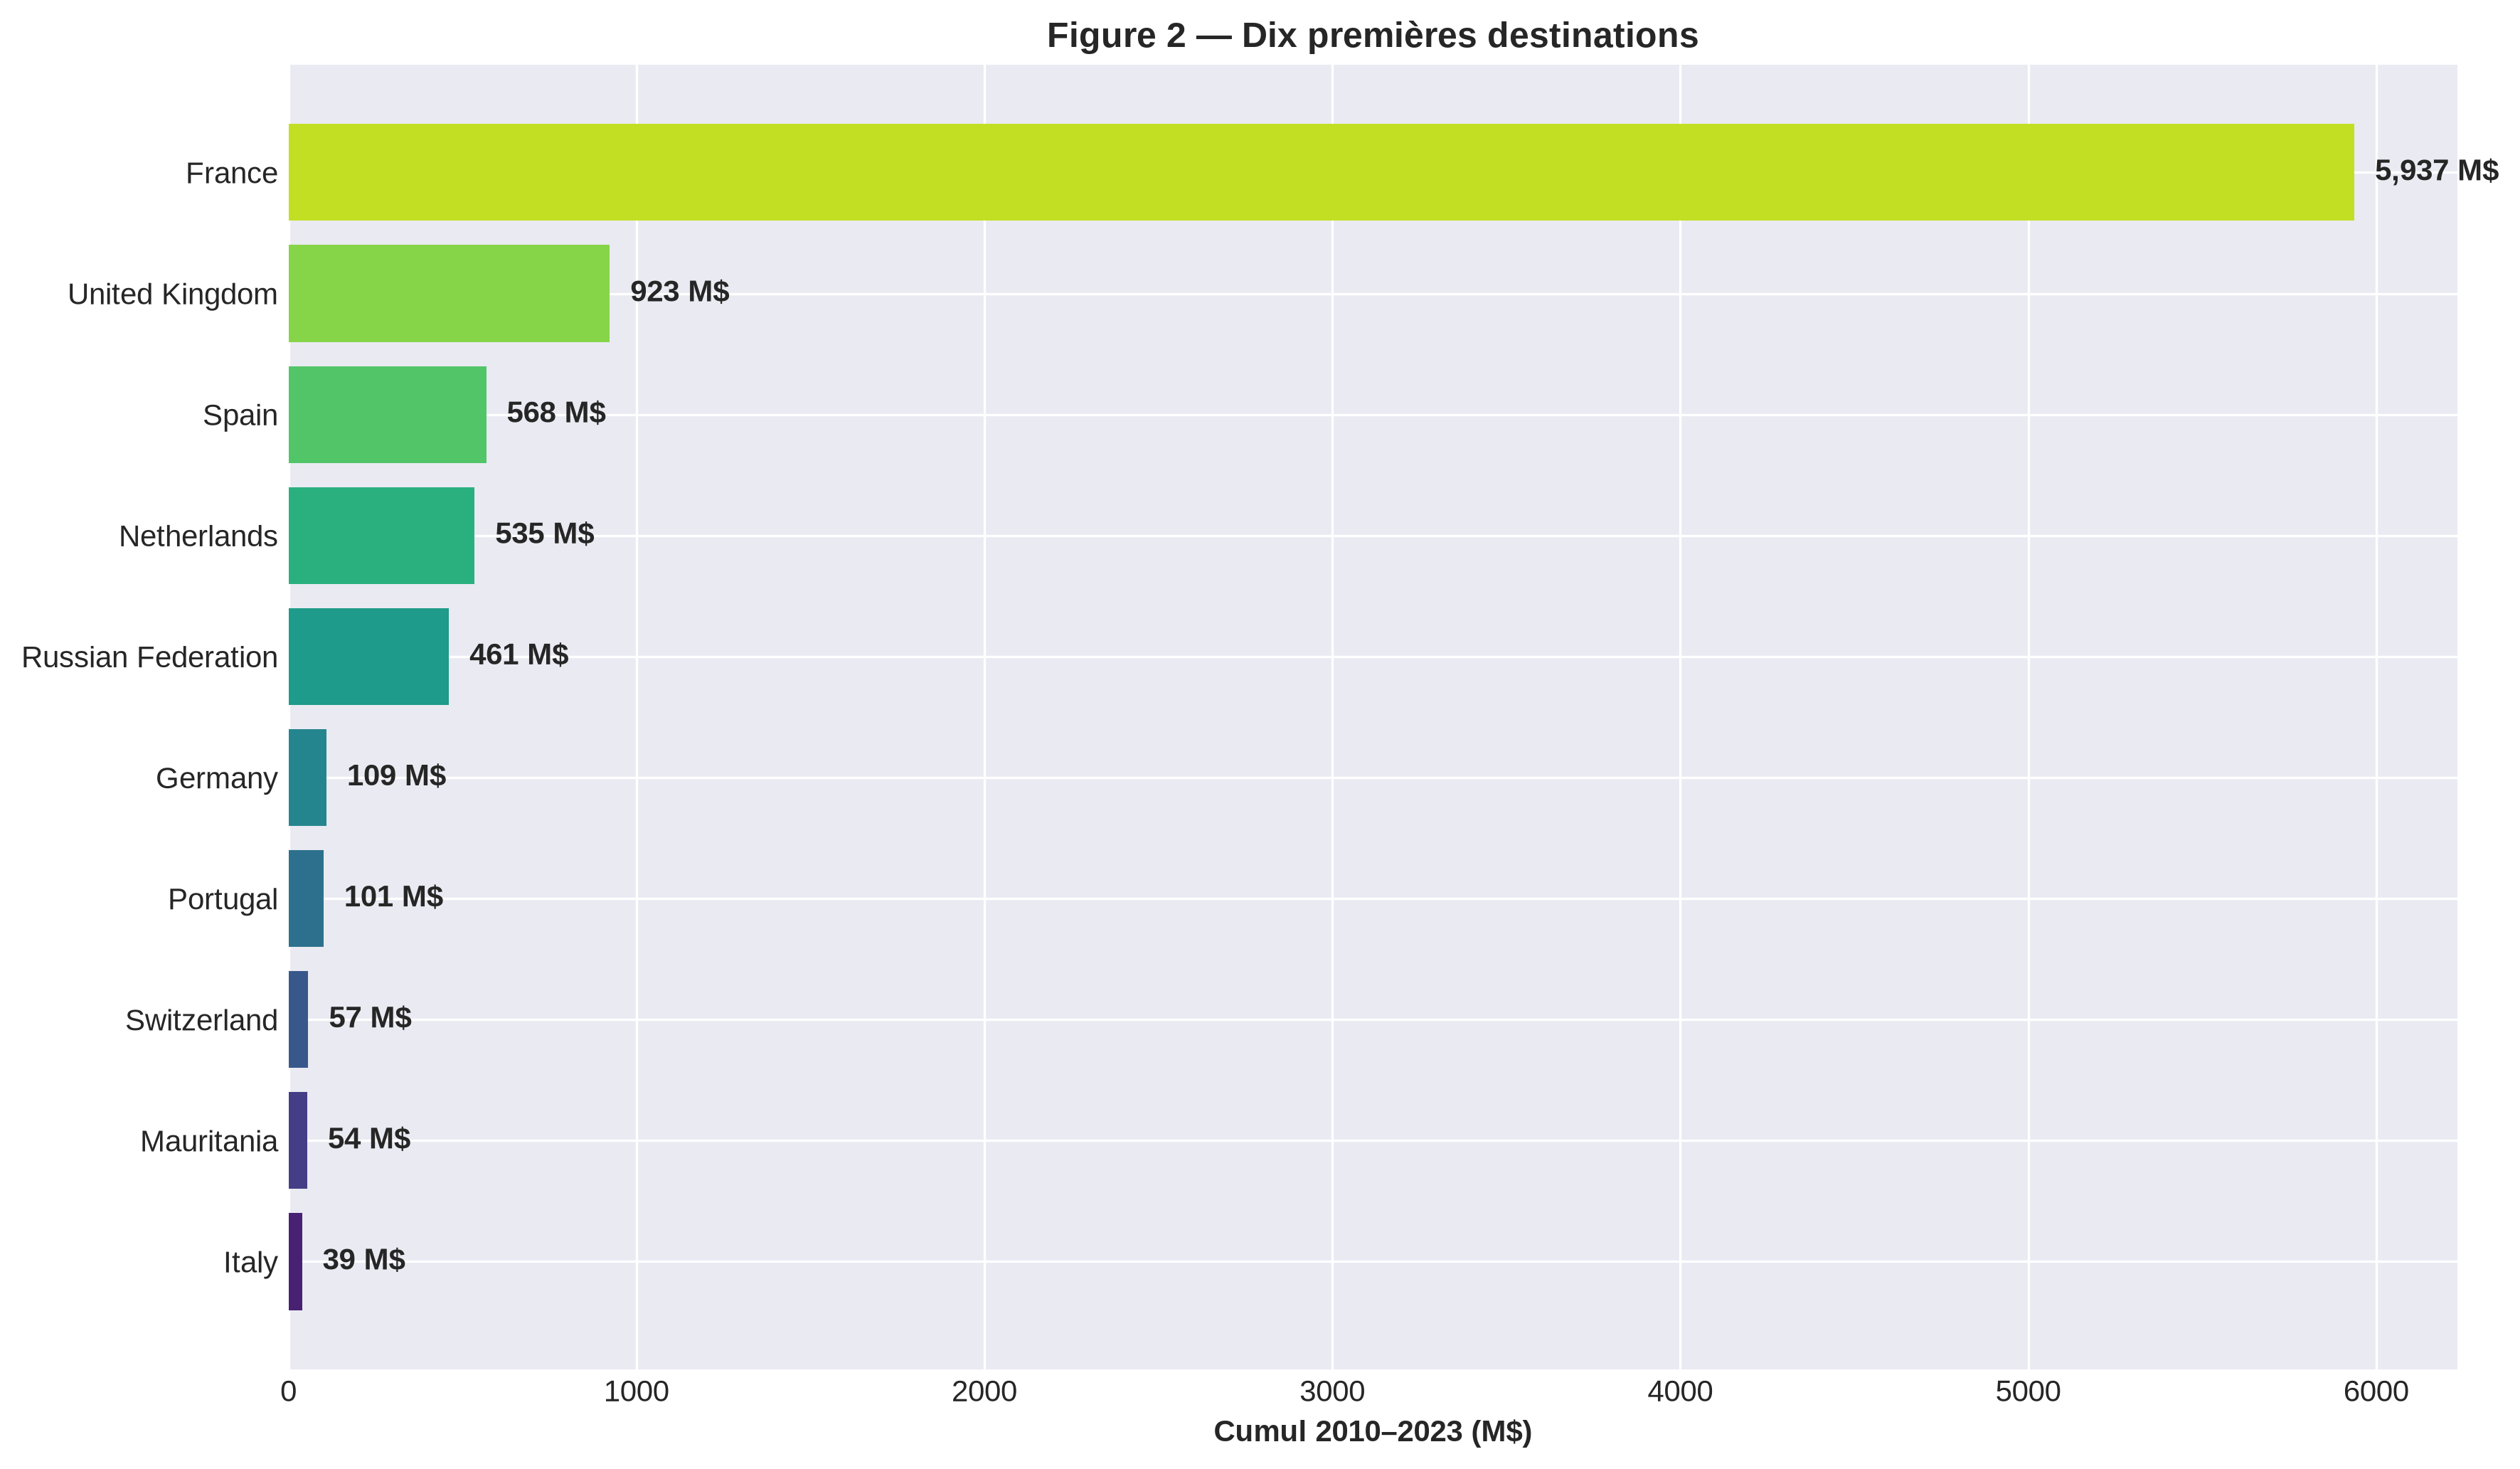
\includegraphics[height=0.60\textheight,width=\textwidth,keepaspectratio]{../figures/fig2_top10_destinations.png}
  \vspace{0.2em}

  \begin{itemize}
    \item La France domine avec 66,4\,\% du total cumulé ($5\,937$\MUSD).
    \item Royaume-Uni 10,3\,\% ; Espagne 6,4\,\% ; Pays-Bas 6,0\,\% ;
          Russie 5,2\,\%.
    \item Les cinq premiers marchés concentrent 94,2\,\% des exportations.
  \end{itemize}
  \src{Source : UN Comtrade (figure~2 du rapport).}
\end{frame}

\begin{frame}{Analyse exploratoire : droits NPF et flux}
  \centering
  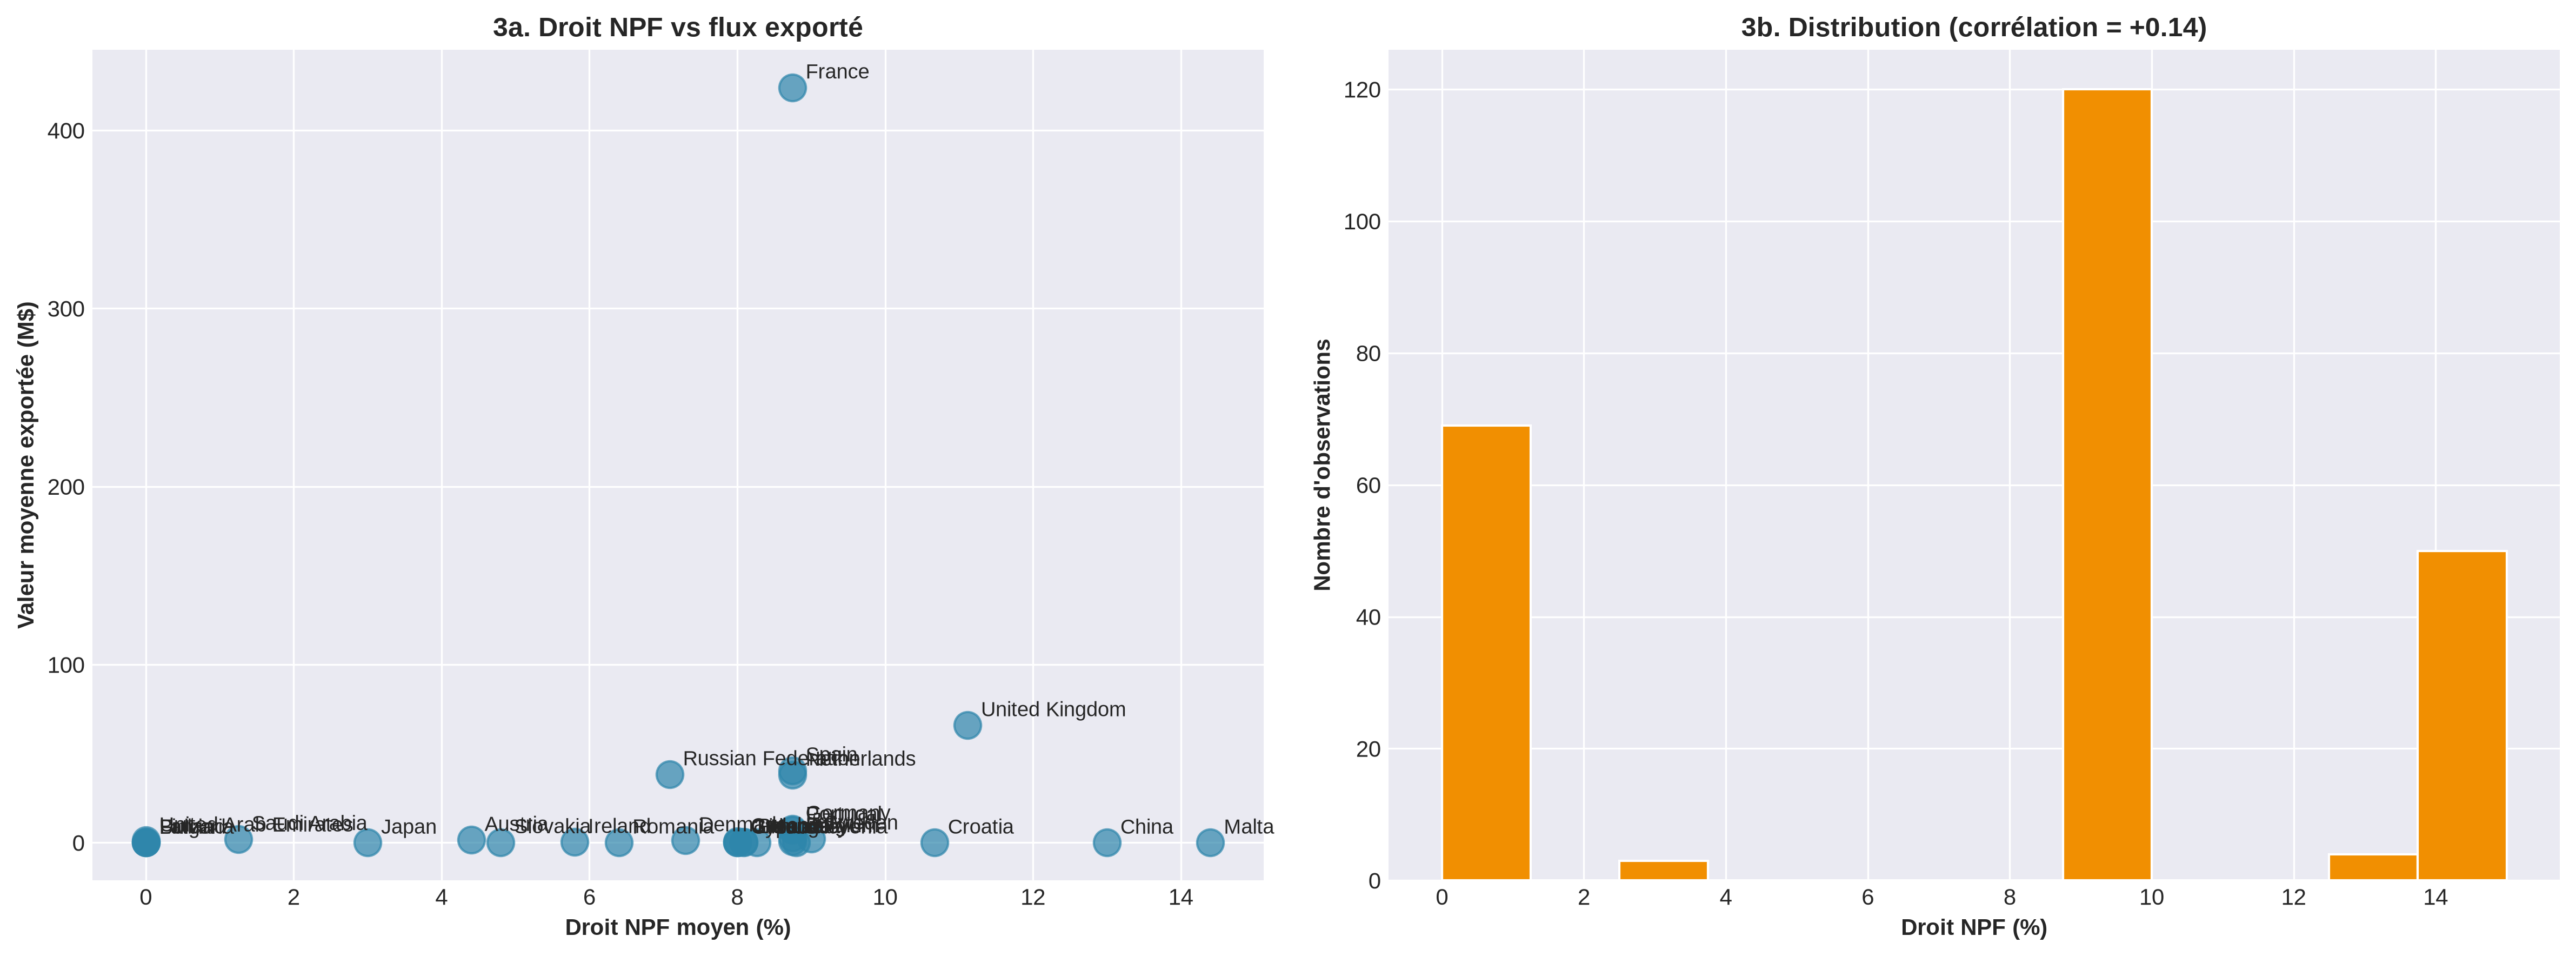
\includegraphics[height=0.60\textheight,width=\textwidth,keepaspectratio]{../figures/fig3_correlation_tarifs.png}
  \vspace{0.2em}

  \begin{itemize}
    \item Corrélation droit NPF / valeur exportée : $\mathbf{+0{,}14}$
          sur 31 partenaires couverts.
    \item Signe \emph{positif} : les marchés à NPF élevé ne reçoivent pas
          moins de flux — résultat contraire à H1.
    \item Les droits se concentrent sur des paliers (0 / 8,8 / 14,4\,\%) :
          effet de régime, pas de gradient continu.
  \end{itemize}
  \src{Source : WITS / UNCTAD TRAINS, HS 070200 (figure~3 du rapport).}
\end{frame}

\begin{frame}{Analyse exploratoire : zones et part de marché}
  \centering
  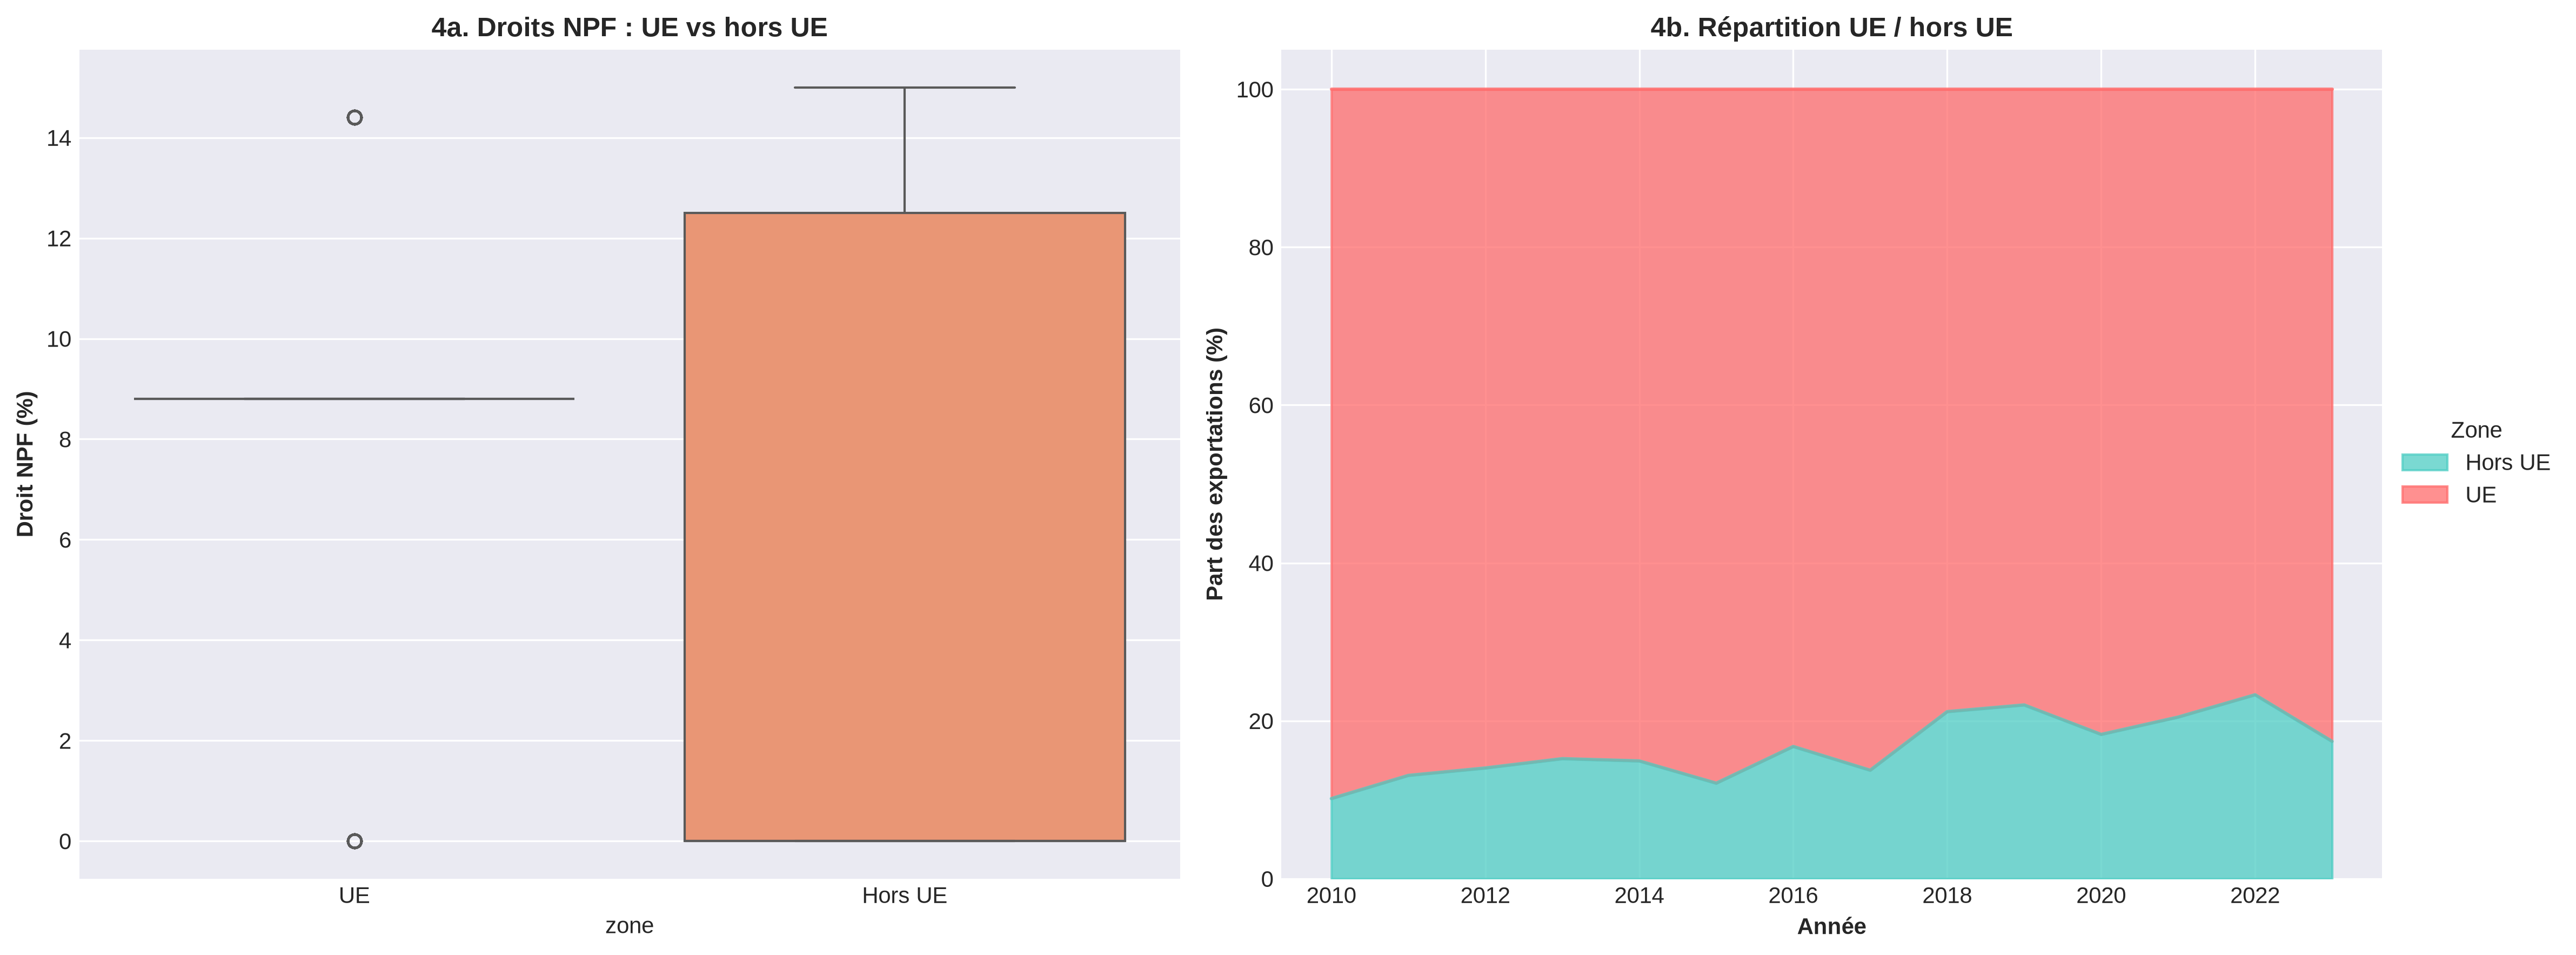
\includegraphics[height=0.46\textheight,width=\textwidth,keepaspectratio]{../figures/fig4_distribution_tarifs.png}
  \vspace{0.3em}

  \begin{columns}[T,onlytextwidth]
    \begin{column}{0.54\textwidth}
      \small
      \begin{itemize}
        \item L'UE : NPF médian de 8,8\,\%, de 0 à 14,4\,\% selon la saison.
        \item Hors UE : forte dispersion (Russie 15\,\%, Émirats 0\,\%).
        \item L'UE absorbe 83,4\,\% de la valeur exportée.
      \end{itemize}
    \end{column}
    \begin{column}{0.43\textwidth}
      \small
      \begin{block}{Lecture}
        Le NPF mesure l'appartenance au marché européen, pas la barrière
        subie : le Maroc y entre sous accord préférentiel.
      \end{block}
    \end{column}
  \end{columns}
  \src{Source : WITS et UN Comtrade (figure~4 du rapport).}
\end{frame}

\begin{frame}{Analyse exploratoire : dynamiques et concentration}
  \centering
  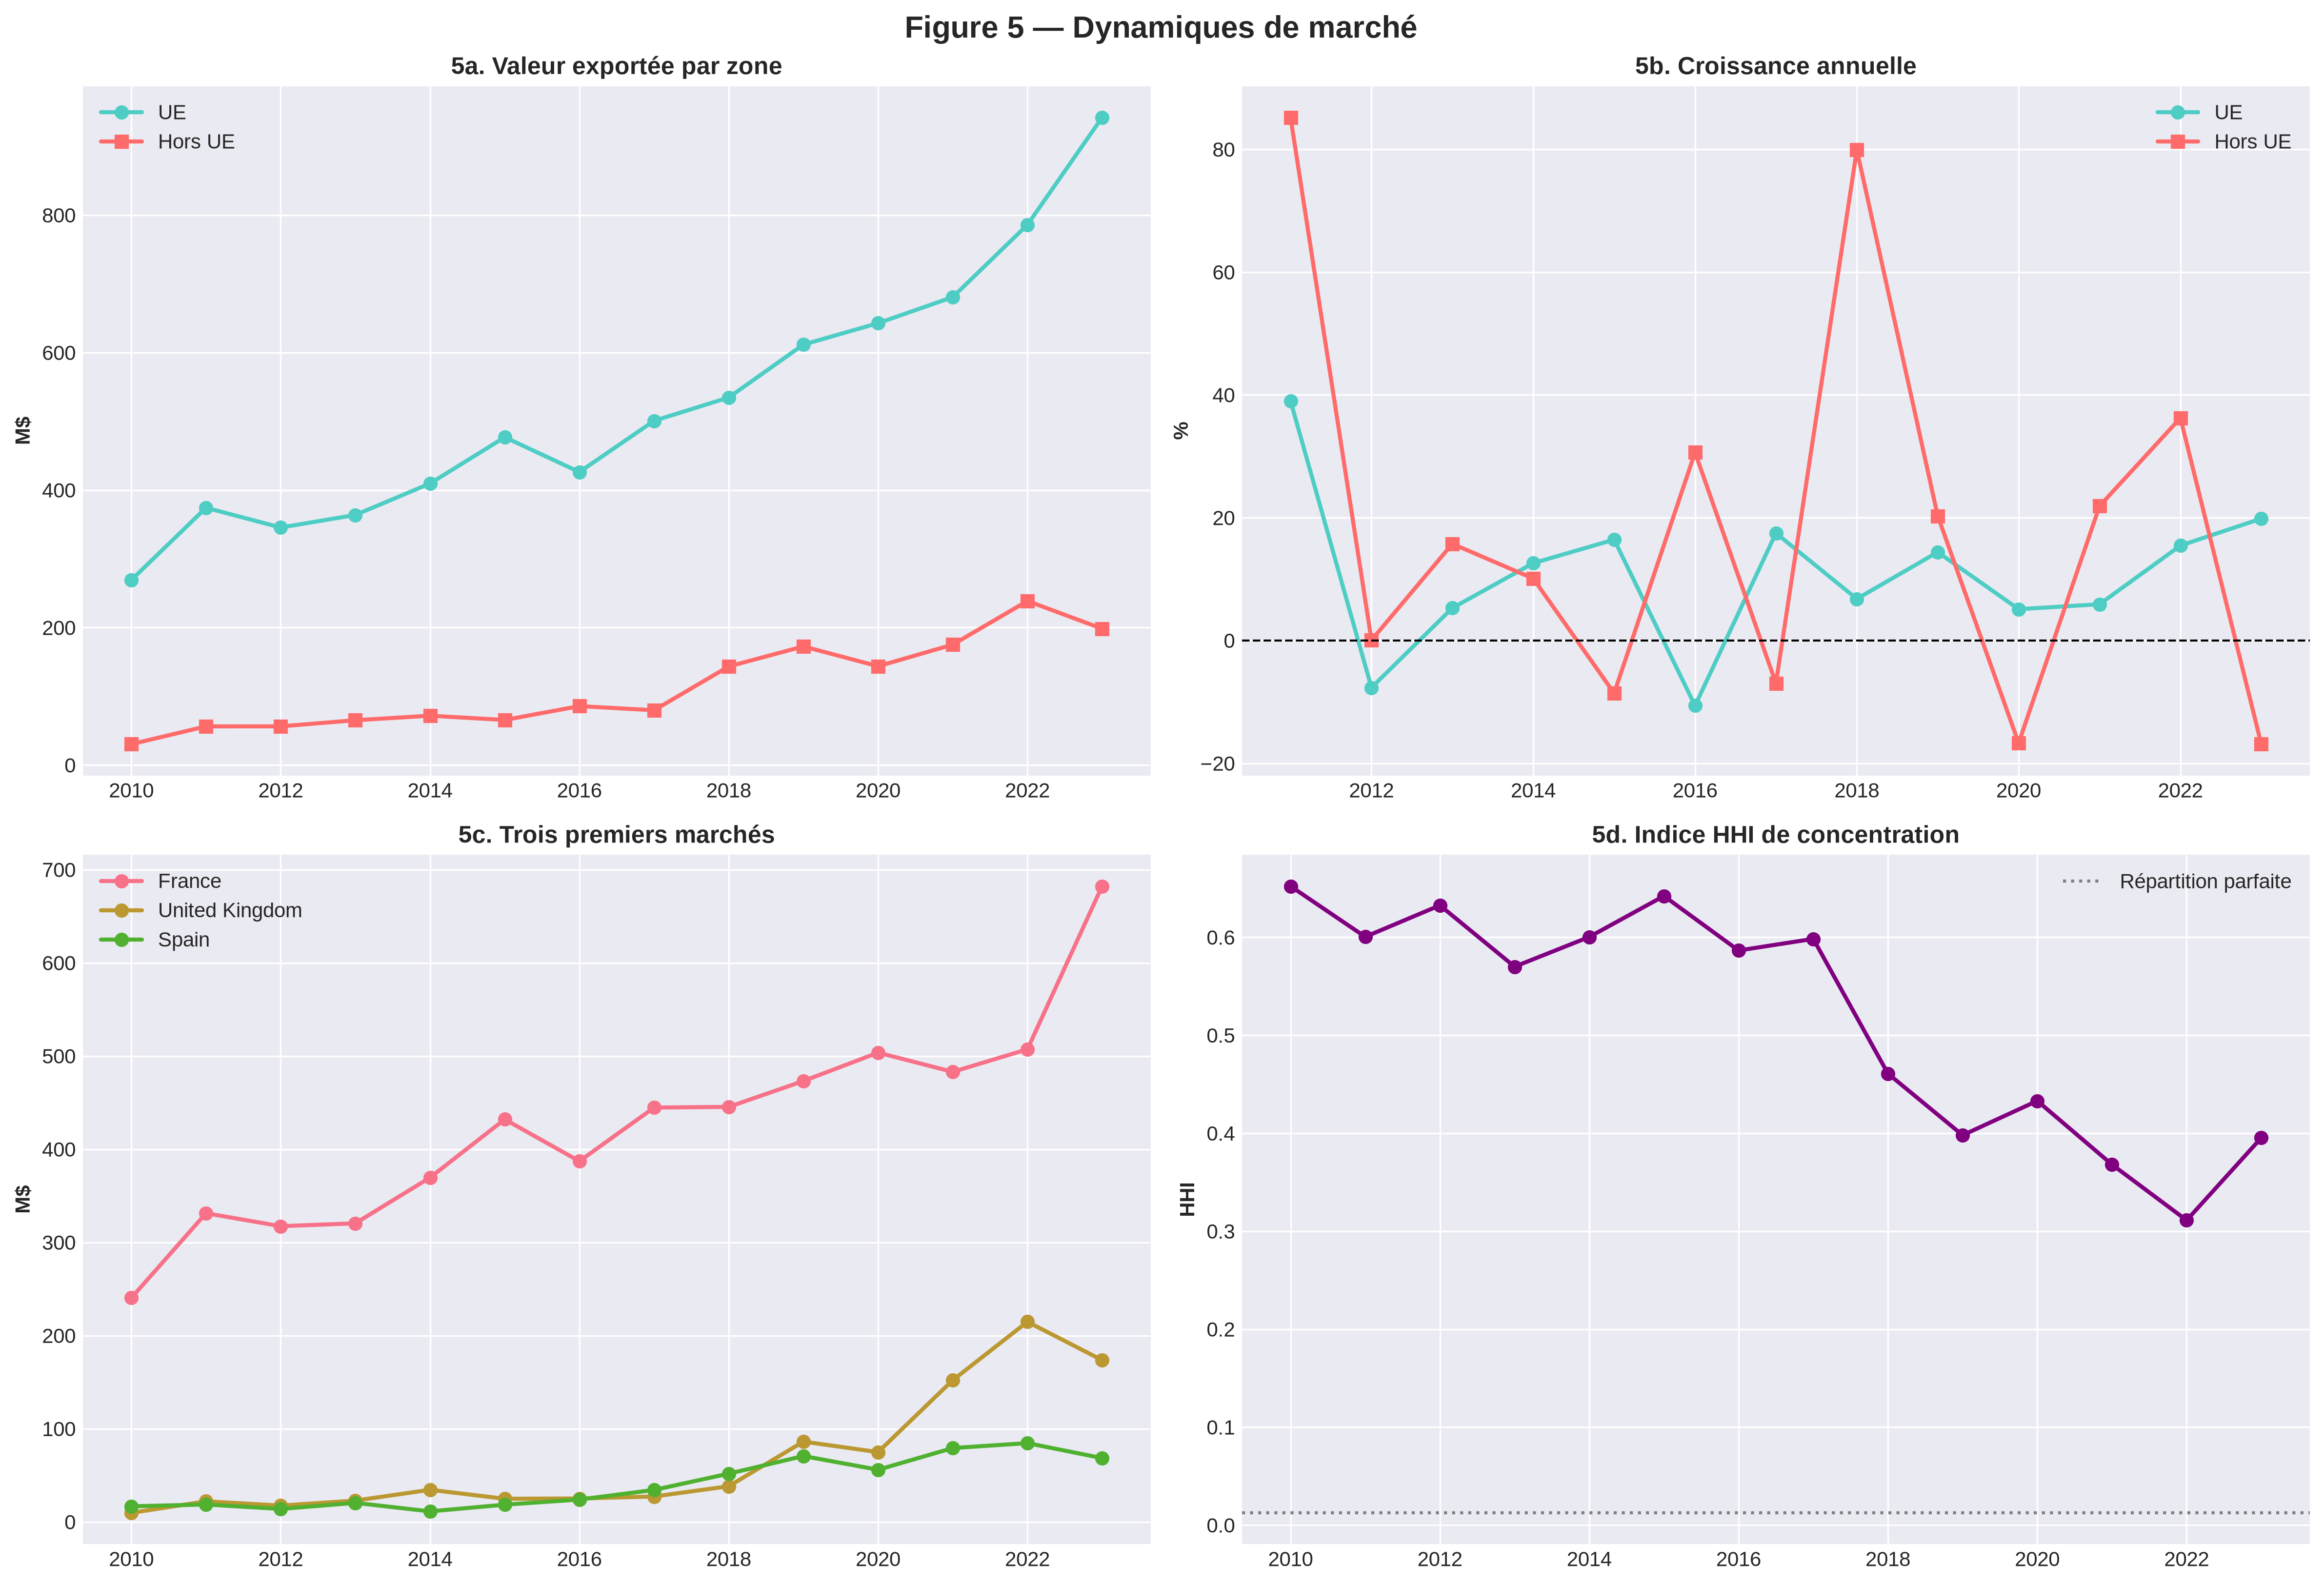
\includegraphics[height=0.58\textheight,width=\textwidth,keepaspectratio]{../figures/fig5_series_temporelles.png}
  \vspace{0.2em}

  \begin{itemize}
    \item Indice HHI : $0{,}652$ (2010) $\rightarrow$ $0{,}395$ (2023),
          contre $0{,}013$ pour une répartition parfaitement égale.
    \item La concentration baisse, mais reste trente fois supérieure à
          l'égalité parfaite.
    \item Royaume-Uni et Russie sont les deux relais de diversification
          les plus crédibles.
  \end{itemize}
  \src{Source : UN Comtrade (figure~5 du rapport).}
\end{frame}

\begin{frame}{Résultats : comparaison des modèles}
  \centering
  \small
  \begin{tabular}{lccccc}
    \toprule
    \textbf{Modèle} & \textbf{MAE val} & \textbf{$R^2$ val} &
    \textbf{MAE test} & \textbf{RMSE test} & \textbf{$R^2$ test} \\
    \midrule
    Référence 1 (moyenne) & -- & -- & 3,519 & 4,318 & $-0{,}002$ \\
    Référence 2 (PIB) & 2,538 & 0,228 & 3,152 & 4,309 & 0,002 \\
    Ridge ($\alpha=1$) & 2,337 & 0,382 & 2,887 & 3,825 & 0,213 \\
    \textbf{Forêt aléatoire} & \textbf{1,878} & \textbf{0,545} &
    \textbf{2,738} & \textbf{3,644} & \textbf{0,286} \\
    \bottomrule
  \end{tabular}

  \vspace{0.9em}
  \begin{columns}[T,onlytextwidth]
    \begin{column}{0.48\textwidth}
      \begin{block}{Forêt aléatoire (meilleur modèle)}
        $R^2 = 0{,}286$ sur le test ; MAE $= 2{,}738$ ; meilleure que la
        référence sur les deux jeux.
      \end{block}
    \end{column}
    \begin{column}{0.48\textwidth}
      \begin{block}{Lecture honnête}
        71\,\% de la variance reste inexpliquée. Deux variables ne
        décrivent pas la répartition des flux : ce modèle est un banc
        d'essai méthodologique, pas un outil prédictif.
      \end{block}
    \end{column}
  \end{columns}
\end{frame}

\begin{frame}{Résultats : ce qui explique les flux}
  \begin{columns}[T,onlytextwidth]
    \begin{column}{0.48\textwidth}
      \textbf{Variables retenues}
      \begin{itemize}
        \item \texttt{log\_gdp} : taille du marché.
        \item \texttt{log\_distance} : distance CEPII.
      \end{itemize}
      \vspace{0.6em}
      \textbf{Variables écartées, et pourquoi}
      \begin{itemize}
        \item \texttt{trend} : un arbre ne peut pas extrapoler une
              tendance ; avec un split temporel, il plafonne à la dernière
              valeur vue.
        \item \texttt{eu\_member} / \texttt{preferential\_agreement} :
              redondants avec l'effet fixe pays, non sourcés.
        \item \texttt{tariff\_npf\_pct} : couverture de 48,6\,\% ; traité
              par une régression dédiée.
      \end{itemize}
    \end{column}
    \begin{column}{0.48\textwidth}
      \begin{block}{Point de méthode}
        La distance est \textbf{constante par pays} : elle agit comme un
        effet fixe pays, pas comme un coût de transport mesuré année par
        année. On ne peut donc pas dire « la distance explique X\,\% ».
      \end{block}
      \begin{block}{Ce que le modèle montre}
        La géographie porte un signal réel (mieux que la référence), mais
        minoritaire : prix, logistique, quotas et saisonnalité manquent.
      \end{block}
    \end{column}
  \end{columns}
\end{frame}

\begin{frame}{Élasticité au droit NPF : un résultat contre-intuitif}
  \begin{columns}[T,onlytextwidth]
    \begin{column}{0.48\textwidth}
      \begin{block}{Estimation log-log (train 2010--2019)}
        {\small
        \[
          \ln(\text{valeur}) = \alpha + \beta\ln(\text{NPF})
          + \gamma\ln(\text{PIB})
        \]
        \[
          +\; \delta\ln(\text{distance}) + \varepsilon
        \]
        }
        \begin{itemize}
          \item $\hat{\beta} = \mathbf{+2{,}22}$, erreur standard $0{,}73$
          \item IC 95\,\% : $[+0{,}78\,;\,+3{,}65]$
          \item 174 observations, 26 partenaires
          \item $R^2$ train $0{,}433$ ; $R^2$ test $0{,}183$
        \end{itemize}
      \end{block}
    \end{column}
    \begin{column}{0.48\textwidth}
      \begin{block}{Pourquoi le signe est positif}
        \begin{itemize}
          \item Les NPF les plus élevés sont ceux de l'UE
                (8,8 à 14,4\,\%).
          \item Or l'UE reçoit 83,4\,\% des flux.
          \item Non pas \emph{malgré} le NPF, mais \emph{grâce} à l'accord
                d'association qui abaisse le tarif effectif.
        \end{itemize}
      \end{block}
      \begin{block}{Conclusion}
        Le NPF mesure l'appartenance au marché européen. H1 n'est donc ni
        validée ni rejetée : elle n'est pas testable avec ces données.
      \end{block}
    \end{column}
  \end{columns}
\end{frame}

\begin{frame}{Classement des marchés (question du catalogue)}
  \begin{columns}[T,onlytextwidth]
    \begin{column}{0.55\textwidth}
      \centering
      \small
      \begin{tabular}{llrl}
        \toprule
        Rang & Marché & NPF moyen & Part \\
        \midrule
        1 & Malte & 14,4\,\% & $<0{,}01$\,\% \\
        2 & Chine & 13,0\,\% & $<0{,}01$\,\% \\
        3 & Royaume-Uni & 11,1\,\% & 10,3\,\% \\
        4 & Croatie & 10,7\,\% & $<0{,}01$\,\% \\
        5 & Suède & 9,0\,\% & 0,3\,\% \\
        -- & France & 8,7\,\% & 66,4\,\% \\
        -- & Russie & 7,1\,\% & 5,2\,\% \\
        -- & Émirats & 0,0\,\% & 0,2\,\% \\
        \bottomrule
      \end{tabular}
    \end{column}
    \begin{column}{0.42\textwidth}
      \begin{block}{Dissociation}
        Les marchés les plus protégés sont économiquement marginaux.
      \end{block}
      \begin{block}{Point de vigilance}
        Le Royaume-Uni est le seul marché à la fois protégé
        (11,1\,\%) et significatif (10,3\,\% des flux). C'est là que se
        joue le vrai enjeu tarifaire post-Brexit.
      \end{block}
    \end{column}
  \end{columns}
\end{frame}

\begin{frame}{Validation des hypothèses}
  \begin{columns}[T,onlytextwidth]
    \begin{column}{0.32\textwidth}
      \begin{block}{H1 --- non testable}
        L'élasticité au NPF est positive ($+2{,}22$). Faute de taux
        préférentiel Maroc dans l'API, la question causale reste ouverte.
      \end{block}
    \end{column}
    \begin{column}{0.32\textwidth}
      \begin{block}{H2 --- partiellement}
        Géographie et PIB portent un signal réel, mais $R^2 = 0{,}286$ :
        l'essentiel de la variance reste inexpliqué.
      \end{block}
    \end{column}
    \begin{column}{0.32\textwidth}
      \begin{block}{H3 --- non tranchée}
        La forêt surpasse Ridge de 0,073 point de $R^2$. Indice faible,
        et les droits sont distribués par paliers.
      \end{block}
    \end{column}
  \end{columns}
  \vspace{0.8em}
  \begin{block}{Synthèse}
    Les données publiques accessibles décrivent bien la concentration et
    classent les marchés, mais ne permettent pas d'identifier un effet
    causal du tarif.
  \end{block}
\end{frame}

\begin{frame}{Recommandations}
  \begin{columns}[T,onlytextwidth]
    \begin{column}{0.32\textwidth}
      \textbf{Pour la recherche}
      \begin{itemize}
        \item Obtenir le taux préférentiel Maroc (WTO TAO, annexes de
              l'accord) : prérequis de toute estimation causale.
        \item Passer en mensuel pour capter la saisonnalité tarifaire
              européenne.
      \end{itemize}
    \end{column}
    \begin{column}{0.32\textwidth}
      \textbf{Pour l'analyse commerciale}
      \begin{itemize}
        \item Suivre l'HHI : baisse de 0,652 à 0,395, mais niveau encore
              très élevé.
        \item Royaume-Uni et Russie : relais de diversification les plus
              crédibles.
      \end{itemize}
    \end{column}
    \begin{column}{0.32\textwidth}
      \textbf{Pour la méthode}
      \begin{itemize}
        \item Ne jamais présenter un droit NPF comme un tarif subi : la
              confusion inverse le signe des conclusions.
        \item Déclarer les manquants plutôt que de les imputer.
      \end{itemize}
    \end{column}
  \end{columns}
\end{frame}

\begin{frame}{Limites et qualité méthodologique}
  \begin{columns}[T,onlytextwidth]
    \begin{column}{0.48\textwidth}
      \begin{block}{Limites}
        \begin{itemize}
          \item Le droit NPF n'est pas le droit subi : l'API WITS ne
                fournit pas le taux préférentiel Maroc.
          \item Couverture tarifaire partielle (48,6\,\% des
                observations, mais 98,2\,\% de la valeur).
          \item Barrières non tarifaires omises : quotas, normes
                sanitaires, traçabilité.
          \item Causalité : les tarifs ne sont pas assignés aléatoirement.
          \item Distance constante par pays : effet fixe, pas coût mesuré.
        \end{itemize}
      \end{block}
    \end{column}
    \begin{column}{0.48\textwidth}
      \begin{block}{Points forts méthodologiques}
        \begin{itemize}
          \item Données réelles, quatre sources publiques, toutes tracées.
          \item Validation temporelle stricte, sans fuite de données.
          \item Quatre modèles comparés, dont deux références naïves.
          \item Hyperparamètres choisis sur validation, test évalué une
                seule fois.
          \item Réponses HTTP en cache : pipeline rejouable.
          \item Graine fixée (42), versions de bibliothèques documentées.
        \end{itemize}
      \end{block}
    \end{column}
  \end{columns}
\end{frame}

\begin{frame}{Conclusion}
  \begin{block}{Ce que montre l'étude}
    \begin{itemize}
      \item Exportations multipliées par 3,8 : $300 \rightarrow
            1\,140$\MUSD{}, soit $+280\,\%$.
      \item Concentration extrême : France 66,4\,\%, top 5 94,2\,\%.
            L'HHI baisse mais reste très élevé.
      \item Le classement par droit NPF montre une dissociation entre
            protection et poids commercial.
      \item Le meilleur modèle atteint $R^2 = 0{,}286$ : la géographie
            porte un signal, mais minoritaire.
      \item L'élasticité au NPF est positive ($+2{,}22$) : la variable
            mesure l'appartenance au marché européen, pas la barrière
            subie.
    \end{itemize}
  \end{block}
  \vspace{0.8em}
  \begin{columns}[T,onlytextwidth]
    \begin{column}{0.48\textwidth}
      \textbf{Perspectives}
      \begin{itemize}
        \item Intégrer le taux préférentiel Maroc et tester H1.
        \item Données mensuelles : saisonnalité tarifaire.
        \item Modèle de gravité structurel avec effets fixes pays et année.
      \end{itemize}
    \end{column}
    \begin{column}{0.48\textwidth}
      \textbf{Message final}
      \begin{itemize}
        \item Les données publiques décrivent bien la concentration, pas
              l'effet causal du tarif.
        \item Savoir ce qu'on ne peut pas conclure fait partie du
              résultat.
      \end{itemize}
    \end{column}
  \end{columns}
\end{frame}

\begin{frame}[plain]
  \centering
  \vfill
  {\Huge\bfseries\color{bleu} Merci de votre attention}
  \vspace{1.2em}

  {\large Questions et discussion}
  \vfill
\end{frame}

\end{document}
